\chapter{Introduction}
\pagenumbering{arabic}
Throughout history, humans have consistently evolved by developing new technologies. Hence, society’s expectations for technology are continually increasing, especially expectations for automation technology, which enables a system or process to operate itself without human intervention \cite{intro_auto}. Automation technology has grown in the past few decades and has gained significant attention. It has grown especially rapidly in the field of mobile
robotics, as it underlies applications such as self-driving cars. Self-driving cars have
captured the attention of many researchers due to their wide range of applications across different fields, such as transportation, logistics, and military \cite{ACs}. Moreover, when self-driving cars reach top-level autonomy, they may save lives by preventing traffic accidents \cite{ACs1}.
\par The autonomy level of self-driving car is ranked by experts on a scale of 0–5 (see figure \ref{fig:autolevel}); level is determined by the extent to which the car can take control from the driver \cite{SAE}. As the autonomy level rises, so does exploitation of localization information, which correspondingly enhances driving safety. In many cases of autonomous driving, the vehicle needs to know where it is to execute a nontrivial task \cite{ACs2}. Therefore, localization is an essential process of autonomy and is required for levels 4 and 5 of autonomous driving.
\begin{figure}[H]
    \centering
    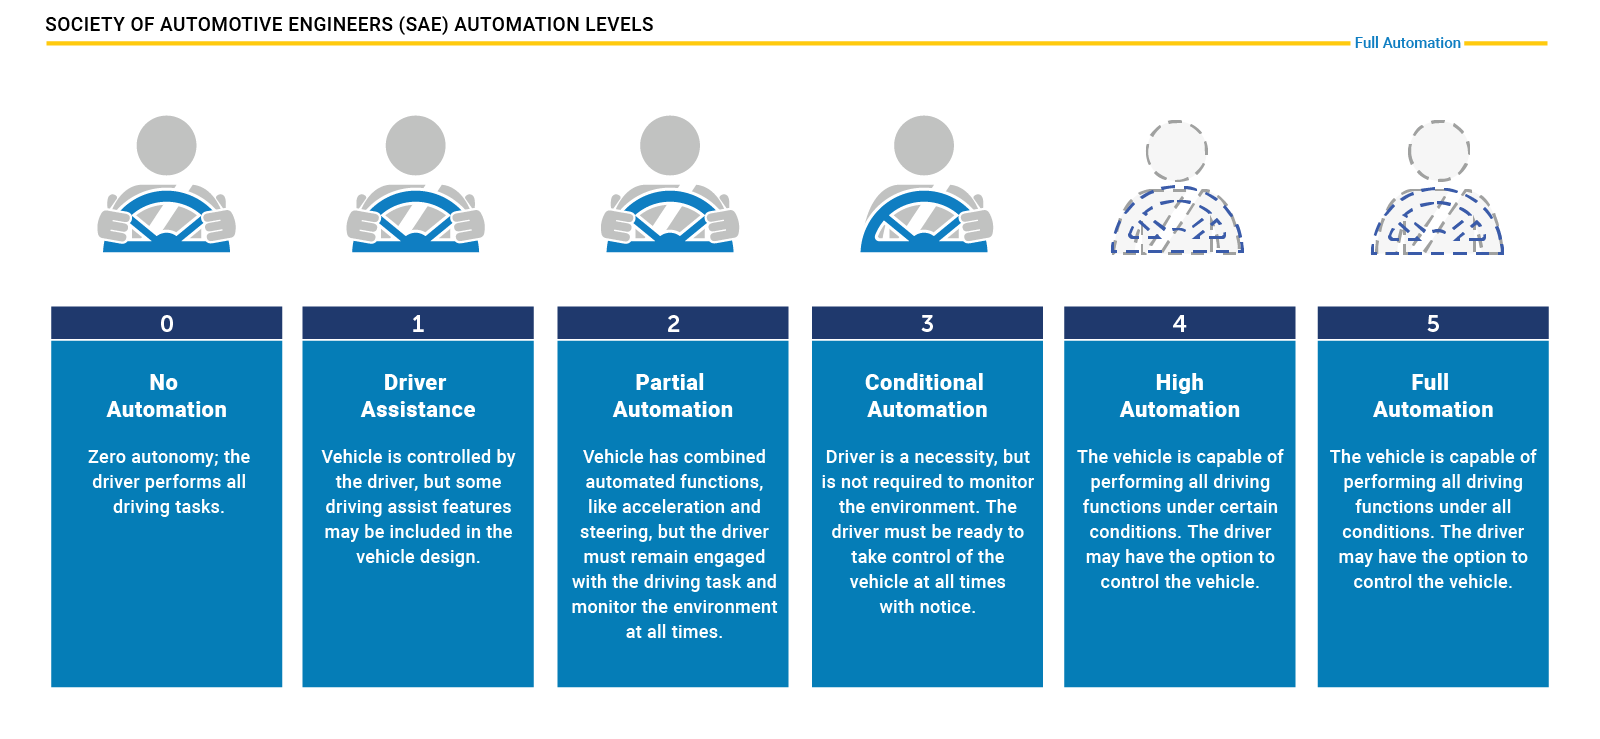
\includegraphics[scale=0.25]{autonomy_level}
    \caption{Five Levels of Vehicle Autonomy}
    \label{fig:autolevel}
\end{figure}

\par The localization problem has recently arisen in mobile robotics, and it is a hot topic addressed by many researchers. They have studied different aspect of localization ranging from low-level techniques, such as wheel odometry and dead reckoning \cite{ACs3,ACs4} to high-level techniques like map-based localization in \cite{ACs2} or \acrfull{slam} in \cite{6D_SLAM,NDT_SLAM}. Following this research, self-driving cars have continued to evolve by employing significant amounts of hardware and software that are not used in ordinary cars. For example, they use several sensors (e.g., \acrfull{lidar} and \acrfull{radar}) to perceive the environment and make decisions about vehicle control with intelligent programs.

\section{Motivation}
\par For the purpose of researching autonomous mobility, there is a vehicle platform, which is called MIAcar, have been developed under CERMcity project at  German Research Center for Artificial Intelligence (DFKI) GmbH. Since the ultimate goal of this project is to enable autonomous driving, especially in urban place, localization becomes one of the most important problem needs to be solved. At first glance, usage of the \acrfull{gps} seems to make the localization problem trivial, but in 2004 DARPA Urban Challange \cite{chp2.4}, it has been shown that GPS by itself was not able to fulfill the requirement of the competition. Moreover, it also caused to drive the vehicle off the road. Therefore, it can be easily said that localization problem still exists and it needs to be overcome by a comprehensive solution. Of note, it is important to highlight that the goal of this thesis is not beat any existing approach, instead thoroughly find most optimal localization approach for our project.
\par Taking these into consideration, this thesis aims to discuss different localization techniques, especially map-based techniques, and to address the following questions:
\begin{itemize}
    \item What kind of sensors can be used for self-driving cars?
    \item What techniques may solve the localization problem?
    \item Which methods can provide a precise localization in decimeter accuracy?
    \item Does the method work in real time on a real system? 
\end{itemize}

\section{Goal of the Master's Thesis}\label{goal}
\par The prime goals of this thesis are defined as follows:
\begin{itemize}
    \item Make a research for sensors and localization methods which are commonly used in respect of self-driving car.
    \item Analysis of different localization methods with different sensor configurations.
    \item Apply different localization methods both on simulation and real system in order to evaluate their results in terms of translation and rotation error.
    \item Allow the MIA car (see figure \ref{fig:mia1}) to perceive its environment by provided localization ability for the purpose of autonomous driving.
\end{itemize} 
\par Ideally, our study’s contribution is to demonstrate that localization methods work both theoretically and practically by improving an optimal localization method that is reliable for executing self-driving car control tasks and can be applied in a real system.
\\
\begin{figure}[H]
    \centering
    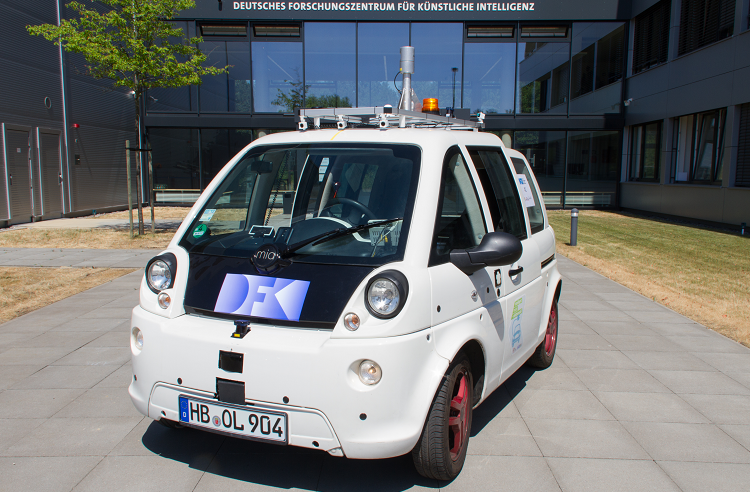
\includegraphics[scale=0.35]{mia1}
    \caption{MIAcar}
    \label{fig:mia1}
\end{figure}
\section{Thesis Organization}
The structure of the thesis is as follows:\\
\\
\textbf{Chapter \ref{chp:2}} describes different sensors and approaches for autonomous cars can be used to provide accurate localization.\\
\\
\textbf{Chapter \ref{chp:3}} covers some algorithms for estimating position of the vehicle in different aspect by using different sensor data.\\
\\
\textbf{Chapter \ref{chp:4}} describes applications of the algorithms from chapter 3.\\
\\
\textbf{Chapter \ref{chp:5}}  presents a quantitative and qualitative comparison of localization algorithms and experimental results.\\
\\
\textbf{Chapter \ref{chp:6}}  concludes this thesis and points out to new idea for future work.